%
% File acl2014.tex
%
% Contact: giovanni.colavizza@epfl.ch
%%
%% Based on the style files for ACL-2013, which were, in turn,
%% Based on the style files for ACL-2012, which were, in turn,
%% based on the style files for ACL-2011, which were, in turn, 
%% based on the style files for ACL-2010, which were, in turn, 
%% based on the style files for ACL-IJCNLP-2009, which were, in turn,
%% based on the style files for EACL-2009 and IJCNLP-2008...

%% Based on the style files for EACL 2006 by 
%%e.agirre@ehu.es or Sergi.Balari@uab.es
%% and that of ACL 08 by Joakim Nivre and Noah Smith

\documentclass[11pt]{article}
\usepackage{acl2014}
\usepackage{times}
\usepackage{url}
\usepackage{latexsym}
\usepackage{graphicx}
\usepackage{subcaption}
\usepackage{mwe}
\usepackage[font=small,skip=0pt]{caption}
%\setlength\titlebox{5cm}

% You can expand the titlebox if you need extra space
% to show all the authors. Please do not make the titlebox
% smaller than 5cm (the original size); we will check this
% in the camera-ready version and ask you to change it back.


\title{A Millennium of Battles}

\author{Marguerite Delcourt\\
  {\small \tt marguerite.delcourt@epfl.ch} \\
  \And
  David Froelicher\\
  {\small \tt david.froelicher@epfl.ch}\\
  \And
Christian Mouchet\\
{\small \tt christian.mouchet@epfl.ch} \\}

\date{\today}

\begin{document}
\maketitle

\begin{abstract}
For centuries, battles have been and still are the most direct action taken by established powers to project or extend their influence. By collecting, processing and analyzing data from the open source, collaborative Wikipedia platform, we are able to better understand how battles were fought throughout the last millennium. In this document, we report our findings from an analysis made over more than 7000 battles. We expose trends in duration and casualties over the years. Additionally, we show that the latter is most important in determining the short-term winner which is not necessarily the long-term one.
\end{abstract}


\section{Introduction}
In 1943, the soviets won the Battle of Stalingrad against the nazis while loosing 800,000 soldiers, twice the number of german casualties. In spite of these heavy losses, this soviet victory is considered as a major strategic turning point that lead to the soviet victory against the nazis' invasion. Human history contains numerous examples such as this one that show the importance and complexity of battles.

While battle-related casualties are far from being representative of all the damage caused by war, they have the particularity of being the result of a strategic and tactical planning, and are therefore worth analyzing. In this work, we make a first step towards understanding the evolution of the way powers wage battle by studying the trends and relationships between multiple battle-related features such as the initial strengths, the number of casualties or the result type of a battle. 

In order to support these observations, we first describe how we collected and processed data on more than 7,000 battles from the English Wikipedia database dump\cite{wikipedia_dump} and provide a short spatial and temporal descriptive analysis of the resulting dataset. Then, we report on our findings observing trends in duration, number of casualties and how indecisive the battles tends to become over the last thousand years. We isolate the adversary losses as a critical feature determining probability of victory and show that this is interestingly not the case for longer-term victories. Lastly, we compute cumulative time spent in battle for each of our extracted belligerents and provide a ranking of the most warlike ones.  


\section{Related works}
The Uppsala University has a Conflict Data Program (UCDP) which is the oldest and biggest provider of war related data. It is considered as the global reference in terms of armed conflicts studies. Even though this ongoing project operates at a much larger scale than ours we can find some correlations. For instance both our plot and their article show that the number of battle related deaths peaked from 1998 to 2001, remained fairly flat until approximately 2012 and increased since then. Our data is more noisy making it harder to see the general trends but peaks are consistent with the UCDP data.
Another interesting similar work is from the article "War and Peace" from the ourworldindata.com website. Just like them, we can notice that the past was not more peaceful, indeed a lot of battles took place between 1500 and 2000. We often think that the world has more conflicts now than in the past but data shows that this is not true, this thought is the mere consequence of our human memory that is less reminded of past conflicts than present times ones. Like them, we notice that the number of battles was very high in the 1900-1950 time period, which is consistent with WW2 and that the world has been very peaceful in the second half of the 20th century. Their results for the number of international battle deaths in the 20th century is also consistent with our findings. Namely we observe that the major peaks of casualties are in 1910-1920 and 1935-1950 time ranges, these values are easily explained by the first and second world wars.
However we also have inconsistent values and trends. For instance we observe that the number of war related casualties over time has a tendancy to go down, while it is not the case from the UCDP database. We explain this by the fact that we consider battle related deaths only while they also consider extra battle but within war deaths such as collateral civilian bombarding.


%ref1: http://pcr.uu.se/digitalAssets/667/c_667494-l_1-k_battle-related-deaths-by-type-of-conflict--1989-2016.pdf
%ref2: https://ourworldindata.org/war-and-peace/

\section{Data collection and  processing}
Given the semi-structured nature of our base dataset, data collection was a significant part of our work. The task was to extract clean and normalized features for each battle related page in the English Wikipedia dump file ($\sim $44 GB). Based on the assumption that the data collection would certainly be an iterative process, we split our pipeline in three steps, enabling each of them to be ran separately and avoiding larger scale computation to be required at each iteration.

\subsection{Page extraction}
The first pipeline step is the only one to be run on the cluster. It performs the page selection based on a regular expression matching of the page title, and outputs a consolidated JSON file containing all selected pages. By avoiding further processing at this step, we effectively reduced our dependency on the cluster, the output being already small enough for local processing ($\sim $123 MB, 27k pages, which was way beyond our initial estimate of 10k).

\subsection{Field extraction}
We leverage on the presence of an \textit{infobox} in most of the battle-related pages. This pipeline step looks for it in the page's source code, which is written using the Wikitext\footnote{https://www.mediawiki.org/wiki/Wikitext} markup language. The syntax generating the \textit{infobox} template\footnote{https://www.mediawiki.org/wiki/Help:Templates/fr} provides a \textit{key}-\textit{value} set for each battle where the keys are conveniently standardized (e.g. \textit{date}, \textit{combatant1}, \textit{combatant2}, \dots).   Values, however, are free text fields, usually containing Wikitext, and natural language formatted for humans. For this reason we qualified our dataset of being semi-structured. The output of this part is a file containing one JSON per battle, with its extracted \textit{key}-\textit{value} set, thus reducing the size to $\sim $14 MB. The number of pages where an \textit{infobox} could be found was 7486, which is within our initial range estimate, and still comfortably large. It appeared that many pages were in fact redirects, drafts or discussion pages.  

At this point, we were able to evaluate which fields could be turned into features by checking the number of concerned pages and the Wikitext processing feasibility. 

\subsection{Feature extraction}
The last pipeline step consists in turning \textit{key}-\textit{value} pairs from the previous step into clean and normalized features. This was clearly one of the most time consuming part of this project, as each field contained very different types of data and thus had to be considered separately. \\
\textbf{date} is a field of primary importance because we initially proposed to analyze the duration of battles. The main difficulty was to deal with many representations of date ranges, as well as dates happening before year 0, which python does not easily accommodate. We decided to ignore such dates after noticing they represent a very tiny fraction of all battles.\\
\textbf{combatant\_\textit{n}}: are the fields containing name(s) of the involved belligerents. Most of the battles have them populated for $n \in \{1, 2\}$, representing the two sides. The difficulty here is twofold: first, the feature type needs to accommodate for coalitions of multiple parties. Second, their affiliation has to be captured at the right level of granularity. We find that a simple yet precise way of learning the state affiliation is to use the flag icons displayed next to the combatant name.\\
\textbf{result}'s content appears to vary a lot from battle to battle, ranging from strait naming of the winner to elaborated aftermath analysis. Consequently, we choose to focus on extracting the victory \textit{type} as it fits well in a categorical variable. In addition, we attribute the extracted result to one of the combatants based on string similarity. This give satisfactory results in most cases, enabling meaningful analysis within sufficiently large sets of battles.\\
\textbf{coordinates} fields are quite rarely populated, which caused problem when studying the spatial distribution of battles. We overcome this issue by extracting page-level geo-tagging data in the previous pipeline step.\\
\textbf{strength\_\textit{n}} contains a summary of side $n$'s strengths, usually in number of soldiers, but often including weapons and assets such as tanks and ships. In most cases, we are able to extract the soldier count or an estimate of it (in case where ranges of values are provided).\\
\textbf{casualties\_\textit{n}} is the most difficult field to extract normalized information from. Even though  it almost always contains a casualties amount breakdown between wounded, killed and captured, the semantical meaning of this breakdown appears very hard to capture. For example, many pages provide breakdowns coming from multiple conflicting sources, when others exhibit phase (or day) based casualties count. On the other hand, conjunction and disjunction used to attribute numbers to the casualty type are often difficult to make sense of. We decide to focus our analysis on one single \textit{casualties\_\textit{n}} feature per combatant, obtained by summing all values (killed, wounded, missing, captured, disappeared).

\section{Descriptive analysis}
While providing exhaustive descriptive analysis for every feature is not feasible within this short report, given their diversity, the reader can refer to the companion notebook. In this section, we focus on analyzing the spatio-temporal coverage of our dataset, as it is important for the rest of the discussion.

\begin{figure}[h]
	\centering
	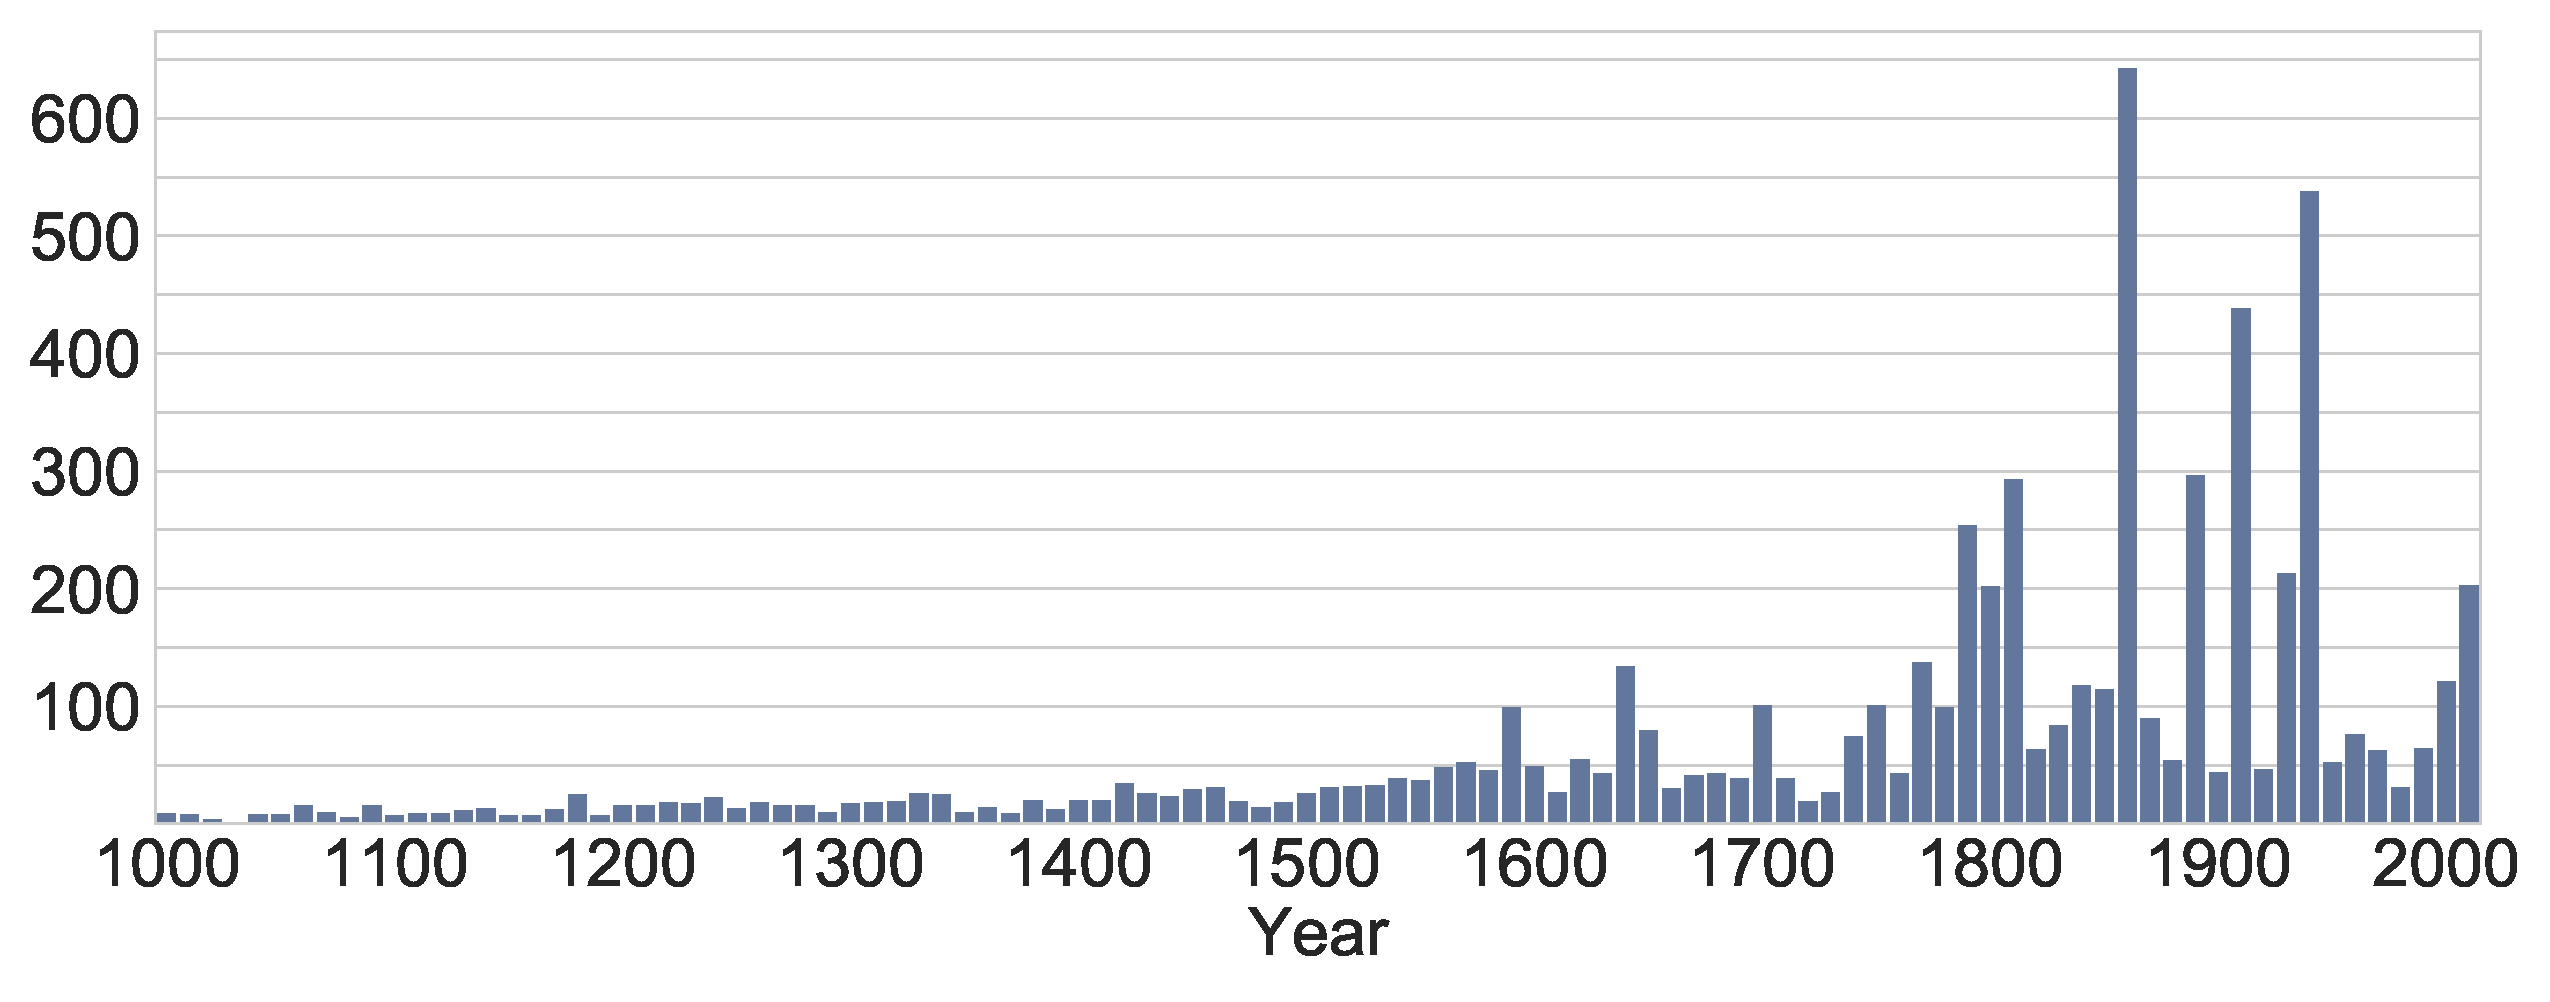
\includegraphics[width=\linewidth]{figures/temporal_coverage.eps}
	\caption{Battle count per decade}
	\label{temporal_coverage}
\end{figure}



\section{Results}
In this Section, we study the information that we can infer from the dataset about the battles and their evolution throughout history. We start by observing how the duration of the battles and the number of casualties progressed during a millennium. Then, we focus on the outcome of the battles, we try to single out the typical features of a victorious combatant and how we can predict or not the result of a conflict. 

\subsection{Duration of the Battles}

We observe that the duration of the battles over the last millenium increased increased almost continuously. In fact, in Figure \ref{fig:durThByCent}, we observe that the order of magnitude of the duration of a battle has never been higher than nowadays. Notice that the average duration of a battle was almost 34 days during the XX$^{th}$ century while it is currently of 64 days in the XXI$^{st}$ century.

 \begin{figure}[h]
	\centering	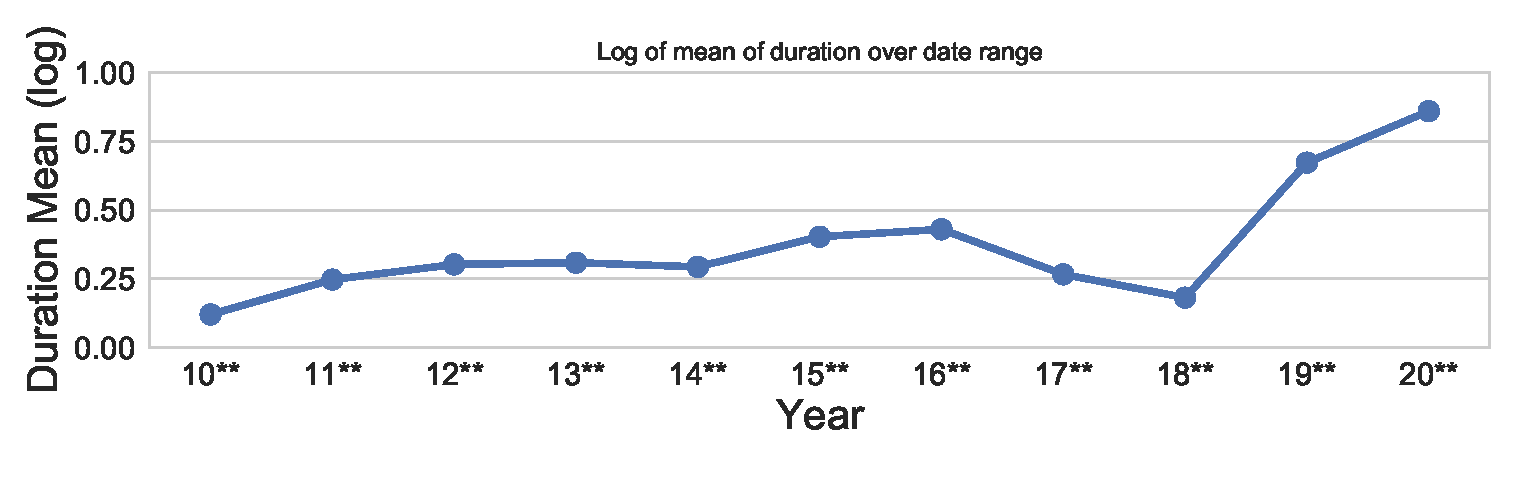
\includegraphics[width=\linewidth]{figures/durThByCent}
	\caption{Mean of the duration of battles in the last thousand years by century on a logarithmic scale.}\label{fig:durThByCent}
	\centering
\end{figure}

\subsection{Evolution of the Casualties}

In Figure \ref{fig:casuPerCent}, we notice that the percentage of soldiers engaged in a battle that are wounded, killed, captured or that disappeared decreases throughout the years. We observe that, following the same trend as shown in Figure \ref{fig:durThByCent} for the battle's duration, the percentage of casualties decreased before increasing in the XX$^{th}$ century. We can infer that in both cases this is due to the world wars because they contain numerous battles which made countless casualties, notably because of technology advances such as aerial forces or gaz attacks.
 \begin{figure}[h]
	\centering	\includegraphics[width=\linewidth]{figures/casuPerCent}
	\caption{Mean of the percentage of casualties in the soldiers.}\label{fig:casuPerCent}
	\centering
\end{figure}

\subsection{Indecisiveness of the Battles}

We observe, in Figure \ref{fig:IndecBattles}, that battles are more indecisive nowadays than they were in the past. In fact, this number (in order of magnitude) is increasing since year 1200 and increased at a higher rate over the last last century. This can be explained by two factors: the first is that battles in the further past were probably often reported by the winner who wouldn't consider it as indecisive. The second is that the two world wars in the  XX$^{th}$ century also contain a lot of strategic and indecisive battles that served a higher or more general goal.
 \begin{figure}[h]
	\centering	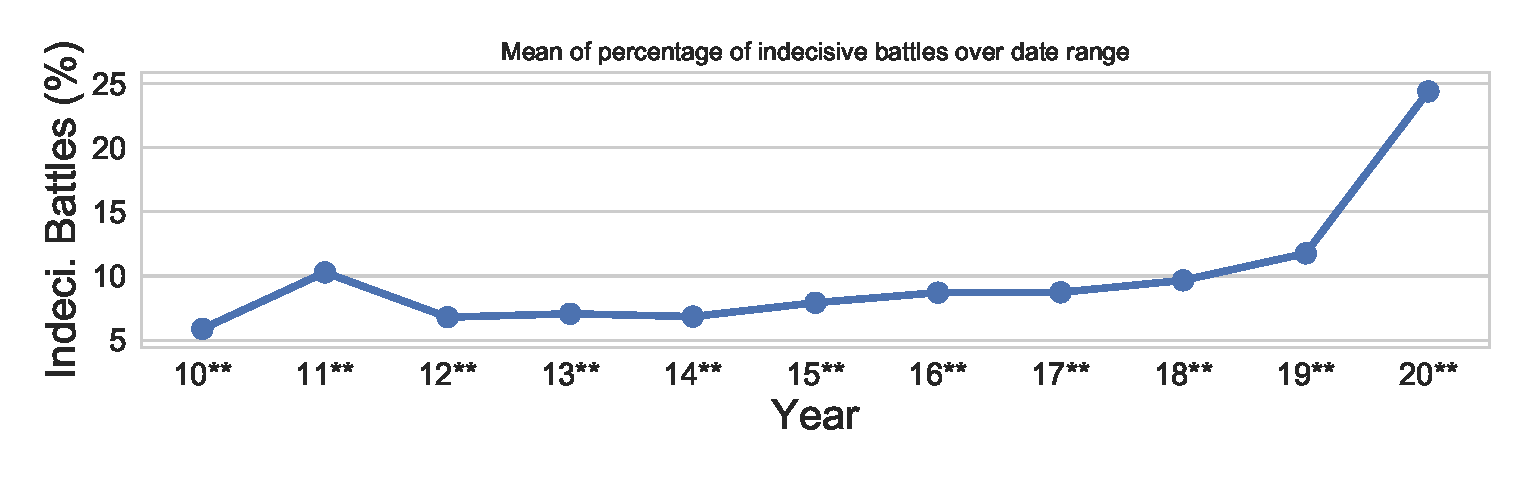
\includegraphics[width=\linewidth]{figures/indThByCent}
	\caption{Mean of the number of indecisive battles over the last thousand years by century on a logarithmic scale.}\label{fig:IndecBattles}
	\centering
\end{figure}

From Figures \ref{fig:durThByCent}, \ref{fig:casuPerCent} and \ref{fig:IndecBattles}, we conclude that battles are longer, make less casualties and are more indecisive over the years. This supports the fact that nowadays the battle's purpose is not only to invade another territory by beating the other combatant. In fact, modern battles seem to be more complicated in the sense that they often serve a higher strategic goal and do not always result in a decisive victory.

\subsection{Outcome of the Battles}

With Figure \ref{fig:victoryAdvantage}, we study the importance for a combatant to have an advantage with respect to the number of casualties (less victims), the number of soldiers (higher strength) and the percentage of casualties among soldiers (casualty ratio). It illustrates the percentage of battles that resulted in a type of victory for a combatant that had an advantage according to one of these features. Our main observation is that the combatant that had less casualties won in almost 80\% of the cases. We noticed that a higher strength resulted in a victory in only less than 50\% of the battles, meaning that in order to predict the winner of a battle, one should simply choose the combatant that suffers less casualties. In order to support our hypothesis, we trained a random forrest classifier on our dataset. Like us, it chose the number of casualties as most important feature to decide the winning side.

We notice that the number of casualties is less important for a strategic victory when the goal is not to inflict more damage to the opponent but to progress towards a more general purpose.
 \begin{figure}[h]
	\centering	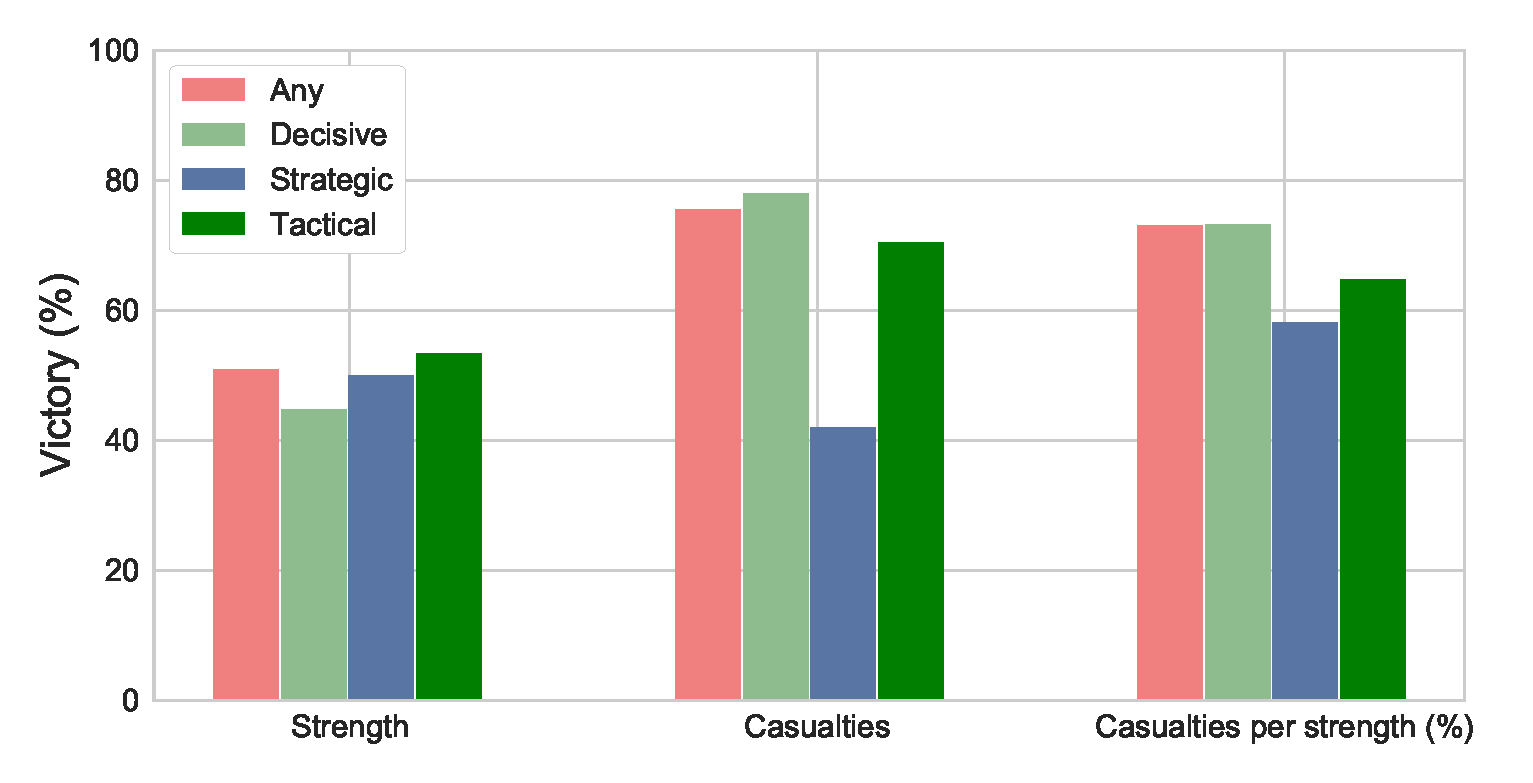
\includegraphics[width=\linewidth]{figures/VictoryAdvantage}
	\caption{Victory percentage with advantage in either strength, casualties or casualty ratio.}\label{fig:victoryAdvantage}
	\centering
\end{figure}

\subsection{Years of Battles per Countries}
In Figure \ref{fig:FightingDurationRanking}, we observe that among all countries in our dataset, France is the one that fought the most. Nevertheless, the United States, which are a major actor in the international history of battles, were only created in 1776 when they proclaimed their independence. Thus, it is interesting to do the same ranking starting from this year. 
 \begin{figure}[h]
	\subfigure[]{\includegraphics*[width=0.5\linewidth]{figures/YearsFightingRanking}} 
	\hspace{-0.4 em}
	\subfigure[]{\includegraphics*[width=0.5\linewidth]{figures/YearsFightingRankingModern}}
	\vspace{-0.1 em}
	\caption{Cumulated duration of battles engagement per country. From 100 in (a) and from 1776 and the United States independence in (b).} 
	\label{fig:FightingDurationRanking}
\end{figure}
 These results tend to support the common belief that the United States are always in war. In fact, as we observe in Figure \ref{fig:USAFightingTimeline}, they were engaged in a at least one battle per year for more than 150 years in 242 years of existence.
 \begin{figure}[h]
 	\centering	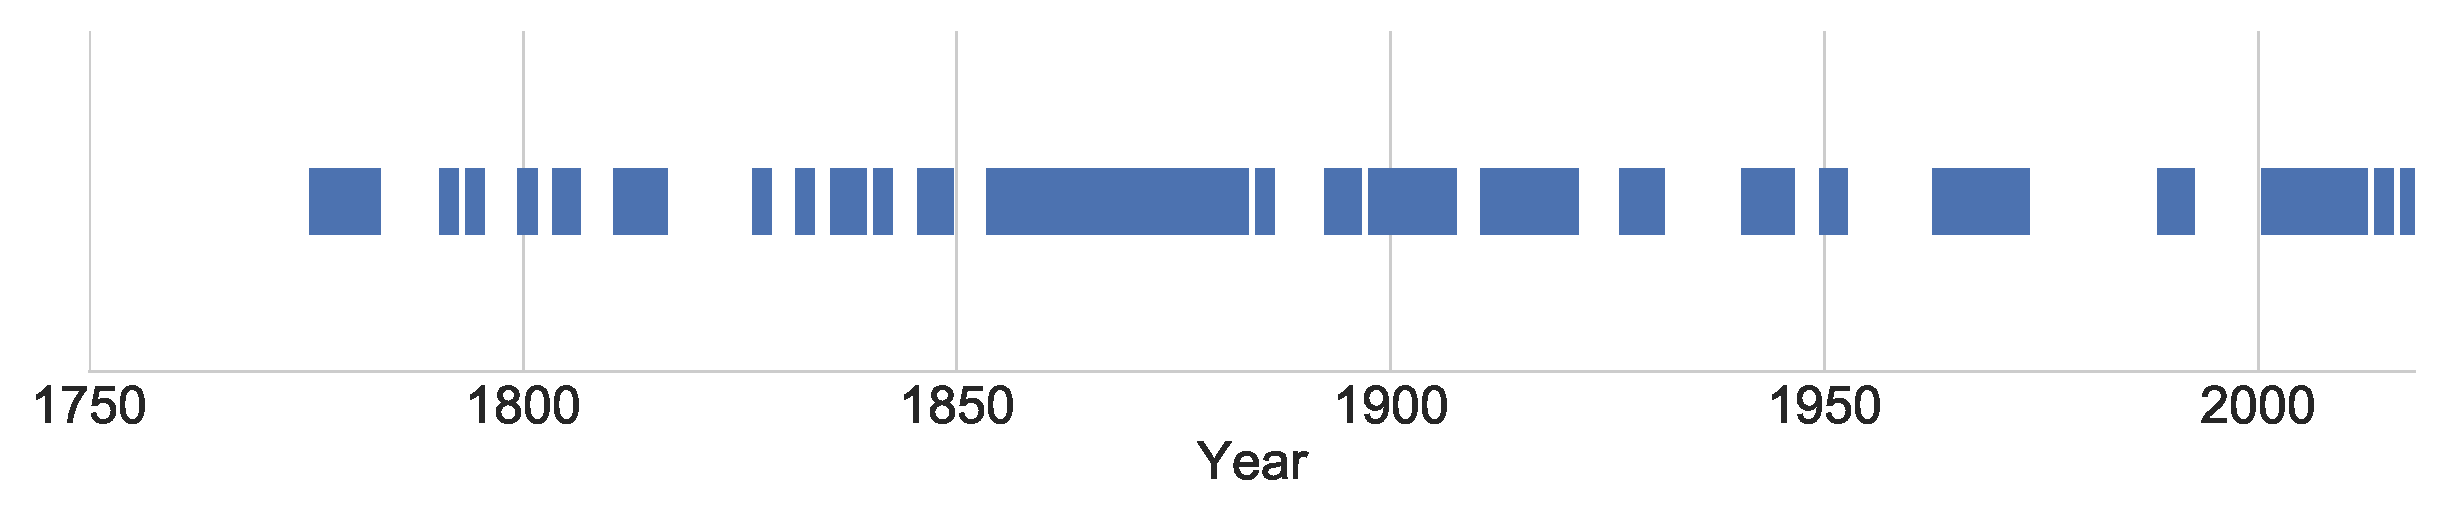
\includegraphics[width=\linewidth]{figures/USAFighting}
 	\caption{Timeline of the USA engagement in battles.}\label{fig:USAFightingTimeline}
 	\centering
 \end{figure}



\section{Conclusion}
In this report, we have collected and processed the data from Wikipedia in order to compile a comprehensive and usable dataset on battles throughout the last millennium. We have shown that battles have become lengthier and more complex, with the probably increasing difficulty of achieving tactical and strategic goals resulting in more indecisiveness. We also pointed out that, while the number of battle-related casualties decreased, the casualties-to-strengths ratio remained almost constants, and that these two statistics are critical for the outcome of the battle, even though there are not enough to achieve a major strategic victory.

\end{document}
